\begin{figure}
\begin{center}
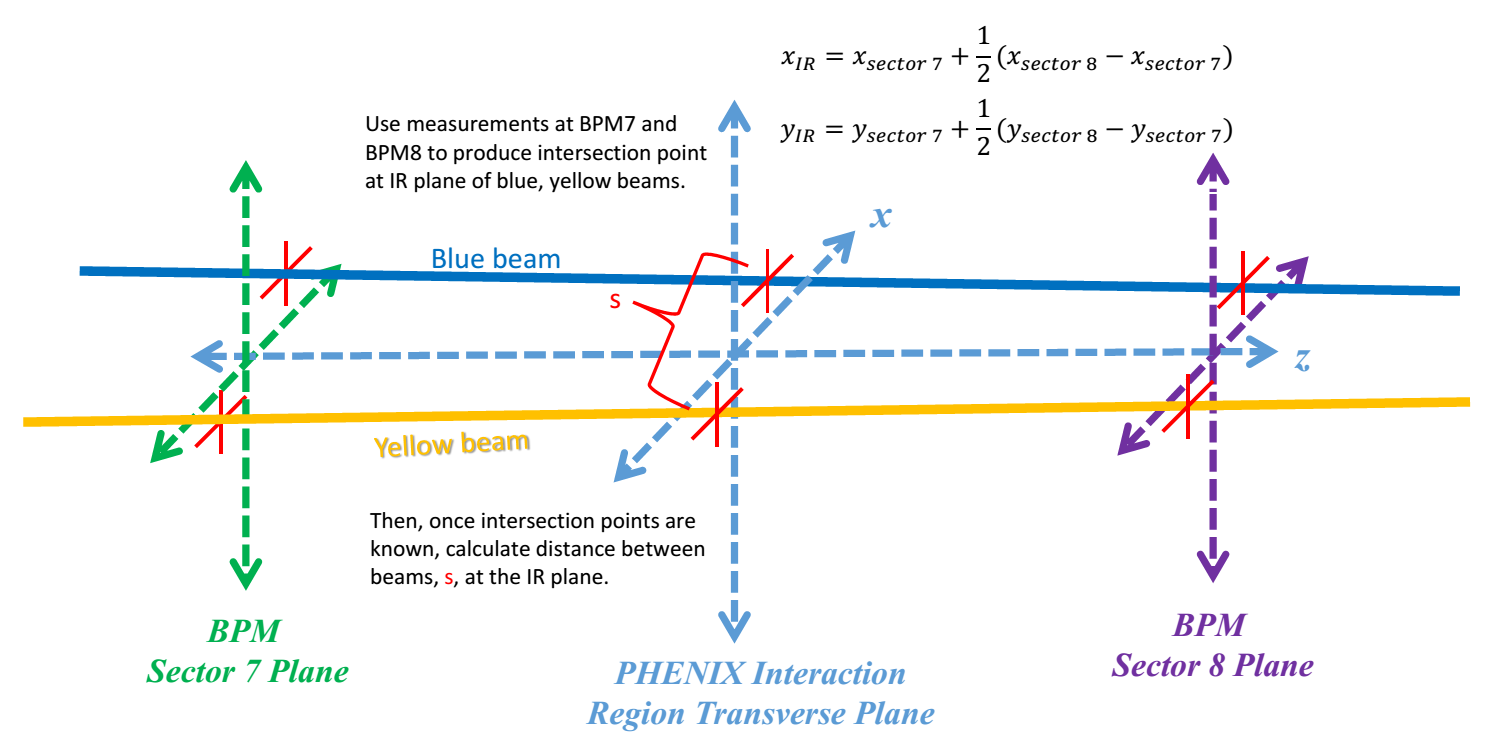
\includegraphics[width=1.0\linewidth]{../DataStreams/figs/bpm_ir_beam_separation}
\caption{We define three parallel planes, each plane is perpendicular to the beam axis.
The planes are at the Sector 7 BPM, the PHENIX IR, and Sector 8 BPM. We assume that the
two BPM planes are equidistant from the PHENIX IR. We can geometrically solve for a three
dimensional line intersecting all three planes, since we have access, for each beam,
intersection points for a given beam at Sector 7 and Sectro 8. With this information, we
determine the intersection points in the transverse plane in the PHENIX IR, and then use
the two intersection points at the IR plane of the blue and yellow beams to calculate
relative beam separation, in both horizontal and vertical directions.}
\label{fig:bpm_ir_xing_cartoon}
\end{center}
\end{figure}
